\chapter{Attachments}

%%-----------------------------------------------------------------------------------------
%% SECTION
%%-----------------------------------------------------------------------------------------
\section{Parameter Description}
\label{sec:parameter_description}

As mentioned in section \ref{sec:implementation_algorithm}, the proposed visualizations can be configured by a set of clustering parameters, a set of visualization parameters and a few other parameters. We will now provide an overview of all of them.

%%-----------------------------------------------------------------------------------------
\subsection{Clustering Parameters}
\label{sec:clustering_parameters}

\begin{description}
\item [Cluster Count] Determines the number of clusters to be retrieved from the dendrogram (see Fig. \ref{fig:telea-hierarchical_clustering}) and used for visualization. If the dendrogram is a tree, any valid number of clusters is guaranteed to cover the whole data set. If the dendrogram is a forest (see section \ref{sec:analysis_clustering_algorithm}), certain parts of the data set may remain uncovered by the chosen clusters. {\bf Valid values:} \(\bm{[1,S]}\) where \(S\) is the number of vertices of one of the {\it scenes}.
\item [Direction Significance] Determines how large the direction weight coefficient in the error function (see Eq. \ref{eq:clustering_error}) will be. See section \ref{sec:parameter_effect} for details. It is only meaningful in combination with all the other significance parameters\footnotemark. {\bf Valid values:} \(\bm{[0,100]}\)
\item [Magnitude Significance] Determines how large the magnitude weight coefficient in the error function (see Eq. \ref{eq:clustering_error}) will be. See section \ref{sec:parameter_effect} for details. It is only meaningful in combination with all the other significance parameters\footnotemark. {\bf Valid values:} \(\bm{[0,100]}\)
\item [Position Significance] Determines how large the position weight coefficient in the error function (see Eq. \ref{eq:clustering_error}) will be. See section \ref{sec:parameter_effect} for details. It is only meaningful in combination with all the other significance parameters\footnotemark. {\bf Valid values:} \(\bm{[0,100]}\)
\item [Resolution Significance] Determines how large the mesh resolution weight coefficient in the error function (see Eq. \ref{eq:clustering_error}) will be. See section \ref{sec:parameter_effect} for details. It is only meaningful in combination with all the other significance parameters\footnotemark. {\bf Valid values:} \(\bm{[0,100]}\)
\end{description}

\addtocounter{footnote}{-4}
\stepcounter{footnote}\footnotetext{\label{conversion}Here is the conversion between {\it significance} and {\it weight}: Consider {\it significance} values \(s_d,s_m,s_p,s_r \in [1,100]\) and {\it weight} values \(k_d,k_m,k_p,k_r \in [0,1]\). We need \(k_d + k_m + k_p + k_r = 1\), therefore \(k_d = s_d / {(s_d + s_m + s_p + s_r)}\) and similarly for all other weights.}
\stepcounter{footnote}\footnotetext{See footnote \ref{conversion}.}
\stepcounter{footnote}\footnotetext{See footnote \ref{conversion}.}
\stepcounter{footnote}\footnotetext{See footnote \ref{conversion}.}

%%-----------------------------------------------------------------------------------------
\subsection{Visualization Parameters}
\label{sec:visualization_parameters}

\begin{description}
\item [Arrow Height Minimum Scale] Determines the height of an arrow representing the lowest metric value present in the data set. This value will multiply the height of the default arrow (see section \ref{sec:implementation_visualizers}) and therefore does not represent the absolute value of the minimum arrow height. {\bf Valid values:} \(\bm{[0.1,10]}\)

\item [Arrow Height Maximum Scale] Determines the height of an arrow representing the highest metric value present in the data set. This value will multiply the height of the default arrow (see section \ref{sec:implementation_visualizers}) and therefore does not represent the absolute value of the maximum arrow height. {\bf Valid values:} \(\bm{[0.1,10]}\)

\item [Arrow Width Minimum Scale] Determines the width of an arrow representing a cluster with the smallest area out of all visualized clusters. This value will multiply the width of the default arrow (see section \ref{sec:implementation_visualizers}) and therefore does not represent the absolute value of the minimum arrow width. {\bf Valid values:} \(\bm{[0.1,10]}\)

\item [Arrow Width Maximum Scale] Determines the width of an arrow representing a cluster covering the whole data set. This value will multiply the width of the default arrow (see section \ref{sec:implementation_visualizers}) and therefore does not represent the absolute value of the maximum arrow width. {\bf Valid values:} \(\bm{[0.1,10]}\)

\item [Arrow Outwards Color] Determines the color of arrows pointing {\it outwards} (see section \ref{sec:analysis}). {\bf Valid values: Any RGB color}.

\item [Arrow Inwards Color] Determines the color of arrows pointing {\it inwards} (see section \ref{sec:analysis}). {\bf Valid values: Any RGB color}.

\item [Color Metric Outwards] Determines the hue of vertices which are assigned a metric vector pointing {\it outwards} (see sections \ref{sec:analysis} and \ref{sec:analysis-color}). {\bf Valid values: Any RGB color}.

\item [Color Metric Inwards] Determines the hue of vertices which are assigned a metric vector pointing {\it inwards} (see sections \ref{sec:analysis} and \ref{sec:analysis-color}). {\bf Valid values: Any RGB color}.

\item [Color Diff Threshold] In absolute mode (see section \ref{sec:analysis-color})), all vertices with an associated metric vector longer than this value will receive the brightest color. {\bf Valid values:} \(\bm{[1, \infty)}\) (In the MeshDiff UI this is limited by the diameter of the whole scene.)

\item [Disabled Color] The color of vertices which were excluded from the visualization by thresholding. {\bf Valid values: Any RGB color}.

\item [Disabled Threshold Length] All vertices with a shorter associated metric vector will be excluded from the visualization. {\bf Valid values:} \(\bm{[1, \infty)}\) (In the meshDiff UI this is limited by the diameter of the whole scene.)

\item [Disabled Threshold Size] All vertices which are part of a cluster whose area is smaller than this value will be excluded from visualization. {\bf Valid values:} \(\bm{[1, \infty)}\) (In the meshDiff UI this is limited by the diameter of the whole scene squared.)
\end{description}

%%-----------------------------------------------------------------------------------------
\subsection{Other Parameters}

The rest of the parameters comprise the viewing angle and zoom of both {\it scenes} and also the metric type, clustering type and visualization type. They are used to configure the mesh viewer in MeshDiff and they also determine how the \verb+DiffVector+ class is initialized (see section \ref{sec:implementation-framework}).

\begin{description}
\item [Zoom Left \& Right] Determines the zoom factor of the mesh view. {\bf Valid values: Not limited.} (The default value is 1.)
\item [Rotation Left \& Right] Determines the viewing angle of a mesh. {\bf Valid values: Any 4x4 rotation matrix.}
\item [Metric] Determines the metric type used in difference computation. (See section \ref{sec:analysis}.) {\bf Valid values: \{Distance, NormalProjectedDistance\}}
\item [Clustering Type] Determines the type of clustering used in the visualization process. (See section \ref{sec:implementation_clustering}.) {\bf Valid values: \{None, Simple, Signed\}}
\item [Color Visualization] Determines the type of color visualization used. (See section \ref{sec:analysis-color}.) {\bf Valid values: \{None, VertexRelative, VertexAbsolute, ClusterRandom, ClusterRelative, ClusterAbsolute\}}
\item [Arrow Visualization] Determines whether arrow visualization is used. {\bf Valid values: \{True, False\}}
\end{description}

%%-----------------------------------------------------------------------------------------
%% SECTION
%%-----------------------------------------------------------------------------------------
\section{Parameter Loading and Storing}
\label{sec:parameter_load_store}

In this section, we describe how MeshDiff can write its configuration to a file and also read it from a file. First, we will talk about the file format. It is a very simple custom format designed to store key/value pairs and to allow for easy reading and writing. Then we will mention how the process of reading and writing is realized in the code.

%%-----------------------------------------------------------------------------------------
\subsection{Format}

Each file is divided into sections which are delimited by a special line containing the name of the section. What follows are key/value pairs, one pair per line. Here is an example of a full configuration file:

\begin{code}
---Trackball Left---
zoom=1
rotation=1,0,0,0;0,1,0,0;0,0,1,0;0,0,0,1

---Trackball Right---
zoom=1
rotation=1,0,0,0;0,1,0,0;0,0,1,0;0,0,0,1

---Metric---
metric=distance

---Clustering Parameters Arrows---
clusterCount=20
directionSignificance=15
positionSignificance=25
magnitudeSignificance=10
resolutionSignificance=0

---Clustering Parameters Colors---
clusterCount=20
directionSignificance=15
positionSignificance=25
magnitudeSignificance=10
resolutionSignificance=0

---Visualizer Parameters---
arrowOutwardsColor=1,1,0
arrowInwardsColor=0,0,1
colorMetricOutwards=1,0,0
colorMetricInwards=0,1,0
disabledColor=0.3,0.3,0.3
arrowWidthMinScale=0.5
arrowWidthMaxScale=5
arrowHeightMinScale=0.5
arrowHeightMaxScale=3
disabledThresholdLength=0
disabledThresholdSize=0
colorDiffThreshold=10

---Form Settings---
clusteringTypeArrows=None
clusteringTypeColors=None
colorVisualization=None
arrowVisualization=No
\end{code}

All lines which do not fulfill any of the following requirements are ignored:

\begin{itemize}
\item Start with \verb+---+
\item Yield exactly two strings upon split at \verb+=+
\end{itemize}

The format of keys and values is defined by the program.
%%-----------------------------------------------------------------------------------------
\subsection{Loading and Storing}

We have written \verb+ParameterWriter+ and \verb+ParameterReader+ classes which can be used in a similar way other I/O classes are used in C\#.

\verb+ParameterReader+ is initialized with a file path and a section name which is the full delimiting string shown above. Then a \verb+ReadPair()+ method can be called in a loop and key/value pairs are returned as tuples. When there are no more pairs in the given section, \verb+null+ is returned. All objects of this class should be disposed of at the end of their lifetime.

\verb+ParameterWriter+ is also initialized with a file path and a section name and provides two methods: \verb+WritePair()+ and \verb+WriteEmptyLine()+. Both methods write to the given file and they always append to file. Upon the first call, a section of the given name is created and all subsequent calls write key/value pairs under that section. \verb+WritePair()+ can only accept arguments of type \verb+string+. This class also implements the \verb+IDisposable+ interface.


%%-----------------------------------------------------------------------------------------
%% SECTION
%%-----------------------------------------------------------------------------------------
\section{MeshDiff User Documentation}

This attachment is structured differently than the rest of the thesis because it aims to be a standalone introductory text to the purpose of MeshDiff and its structure from a user point of view.

For clarity, each section of this chapter represents an answer to a question the user may ask when consulting the user documentation. The text also addresses the user directly. At the beginning, however, we provide a short introduction of what MeshDiff is.

\subsection{About MeshDiff}

MeshDiff is a graphical program running on Windows operating systems which allows its users to interactively view two homologous triangle meshes\footnotemark in \verb+.ply+ or \verb+.obj+ format and visualize the difference between them. MeshDiff has various color-based, arrow-based and combined visualizations available. Once the user has found a visualization which suits their intentions the best, there are two options of saving the visualization:

\begin{itemize}
\item It can be exported as a \verb+.ply+ file and subsequently loaded in any \verb+.ply+ viewer, for example in a mobile application called MorphoView and  presented in \citet{Pikora}
\item Its configuration can be saved. In this case, MeshDiff can load the configuration and generate the very same visualization under the very same viewing angle later
\end{itemize}

\footnotetext{See footnotes \ref{foot:triangle_mesh} and \ref{foot:homologous}.}

\subsection{How do I begin?}

Once you have two homologous triangle meshes you wish to compare (homologization can be done for example in Morphome3cs), load one of them into the left panel and the other one into the right panel:

\begin{description}
\item [To load the left mesh:] \verb+File > Load Model 1+, and choose the \verb+.obj+ or \verb+.ply+ file you wish to load
\item [To load the right mesh:] \verb+File > Load Model 2+, and choose the \verb+.obj+ or \verb+.ply+ file you wish to load
\end{description}

\subsection{How do I control the view?}

You can view the meshes interactively by clicking and dragging the mouse cursor over them. You can also zoom in and out using the mouse wheel.

By default, when you hover over one of the meshes while controlling the view, you change the view of both meshes at the same time. This is because the \verb+Paired Controls+ toggle is enabled. Click \verb+View > Paired Controls+ to disable it. Mesh views can be controlled separately with this option disabled.

If you want to reset the views of both meshes to their default position, click \verb+View > Reset cam+.

There are other toggles in the \verb+View+ menu, all of which modify the view in a certain way. Here is their description:

\begin{description}
\item [Axes] Draws the \(x\), \(y\) and \(z\) axes into the view for better orientation
\item [Smooth] Interpolates mesh color in triangles to makes the surface look smooth. When disabled, each triangle is assigned only one color
\item [Wire] When enabled, mesh triangles are not filled which results in a wireframe rendering of the mesh
\item [Visualization Wire] A separate wire toggle for arrow visualizations
\item [2-sided] When disabled, only the side of triangles which is assigned a normal is drawn. This is useful for example when rendering half-enclosed meshes of human faces where viewing the face from the ``inside'' creates an unpleasant effect
\item [GLSL] Enables shaders. When shading is computed, meshes look less flat
\item [Ambient] When shaders are enabled, this option adds ambient light. Ambient light is a sourceless light illuminating all parts of the mesh uniformly. In reality, this roughly corresponds to light which has been reflected many times and therefore illuminates even surfaces which are not facing a light source 
\item [Diffuse] When shaders are enabled, this option adds diffuse reflections. Diffuse reflections occur in objects with a rough surface where light is reflected in many unpredictable directions
\item [Specular] When shaders are enabled, this option adds specular reflections. Specular reflections occur in polished objects with a prevalent direction of reflected light. They make the object look shiny
\item [Phong] When shaders are enabled, this option toggles Phong shading. This is an alternative shading algorithm which tries to hide the edges between triangles
\end{description}

\subsection{How do I create a visualization?}

Once you have loaded both triangle meshes and set the view according to your taste, you can create a visualization of the difference between the two meshes. Please, see section \ref{sec:analysis} for a thorough analysis of all the visualization that MeshDiff supports.

Basic configuration of a visualization can be done in the main window of MeshDiff. The \verb+Arrow Visualization+ and \verb+Color Visualization+ dropdowns allow you to choose specific types of both visualizations. You can disable either of them by choosing \verb+No+ and \verb+None+ respectively, but it is also possible to combine them together.

Once the visualization types have been chosen, optional clustering can be added to the visualization process to display more general information. Clustering can be configured independently for both arrow visualization and color visualization. The required clustering type can be set via \verb+Clustering for Arrows+ and \verb+Clustering for Colors+ dropdowns and once a non-empty type is chosen, the corresponding trackbar will become active. The values of the trackbars determine the number of clusters which will be displayed for a given visualization type.

Please note that when selecting the \verb+Signed+ clustering, certain cluster counts do not cover the whole triangle mesh and leave black spots or show no arrows where no clusters have been chosen.

When you are ready, click \verb+Update Visualization+.

\subsection{How do I change clustering parameters?}

If you have selected a certain clustering type for your visualization and are not satisfied with the result, MeshDiff provides a way for you to change the clustering parameters. More on what they are and what their effect is can be found in section \ref{sec:parameter_effect}.

Click \verb+Settings > Clustering Parameters+ to view the following window:

\begin{figure}[h]
\centering
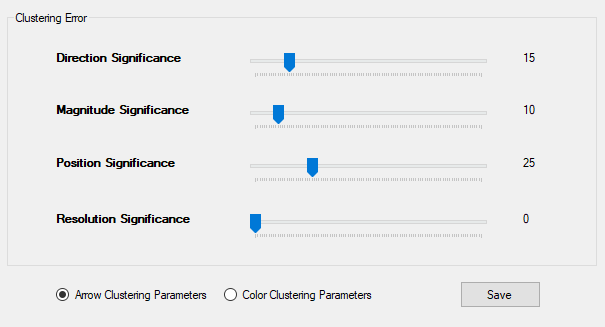
\includegraphics[width=1\textwidth]{./img/meshdiff-clustering_parameters.PNG}
\caption[MeshDiff - Clustering Parameters]{MeshDiff - Clustering Parameters Configuration Window}
\label{fig:meshdiff_clustering_parameters}
\end{figure}

The checked radio button at the bottom signifies which parameters are currently being edited. The trackbar values determine the relative significance, in other words, \verb+Position Significance+ at 80 and with other values at 40 gives the same result as \verb+Position Significance+ at 40 with other values at 20.

Click \verb+Save+ to remember current values.

\subsection{How do I change visualization appearance?}

Appearance parameters, such as colors, arrow size and other can be configured by clicking \verb+Setting > Visualizer Parameters+. The following window will then appear:

\begin{figure}[h]
\centering
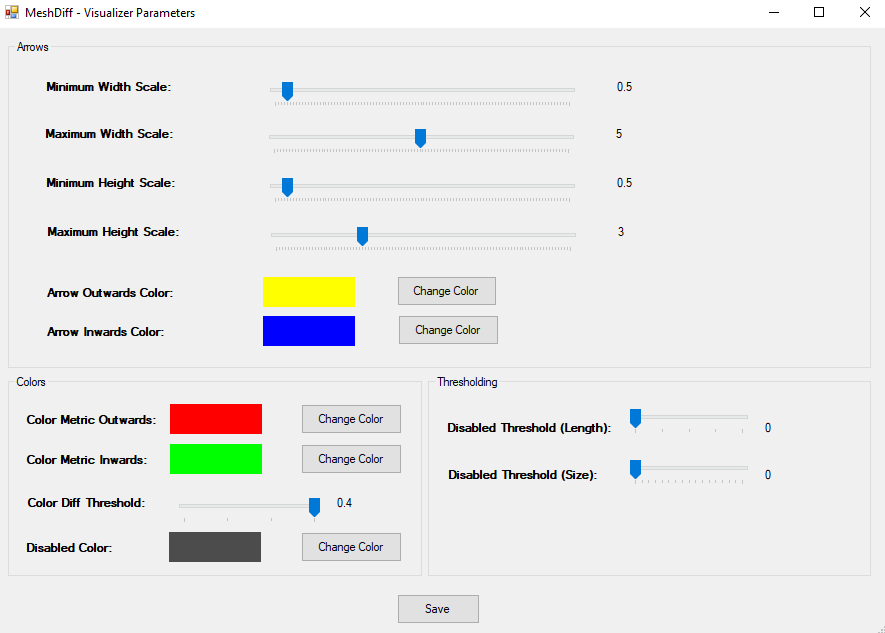
\includegraphics[width=1\textwidth]{./img/meshdiff-visualizer_parameters.PNG}
\caption[MeshDiff - Visualizer Parameters]{MeshDiff - Visualizer Parameters Configuration Window}
\label{fig:meshdiff_visualizer_parameters}
\end{figure}

See appendix \ref{sec:visualization_parameters} for a detailed description of these parameters.

Please note that the maximum range of the threshold trackbars depends on the number of vertices the currently loaded triangle meshes have. It is therefore advisable to configure these parameters after the meshes have been loaded.

Click \verb+Save+ to remember current values.

\subsection{How do I export my visualization?}

MeshDiff is able to export visualizations in the \verb+.ply+ format.

\begin{itemize}
\item To export the left visualization, click \verb+File > Export Visualization 1+
\item To export the right visualization, click \verb+File > Export Visualization 2+
\end{itemize}

When you do that and your visualization contains arrows, you will be asked if you want to export arrows separately (see Fig. \ref{fig:meshdiff_separate_arrows}). By clicking \verb+No+, the complete visualization will be stored in one \verb+.ply+ file. If you click \verb+Yes+, the underlying triangle mesh with a color visualization (if there is one) will be stored in a file called \verb+[chosen name].ply+. The arrows will be automatically stored in a separate file called \verb+[chosen name].arrows.ply+.

\begin{figure}[h]
\centering
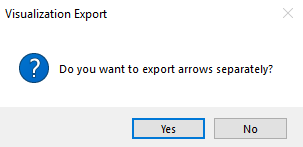
\includegraphics[width=0.4\textwidth]{./img/meshdiff-separate_arrows.PNG}
\caption[MeshDiff - Export Prompt]{MeshDiff - Export Prompt}
\label{fig:meshdiff_separate_arrows}
\end{figure}

\subsection{How do I load an exported visualization?}

Because visualizations are triangle meshes stored in \verb+.ply+ files, they can be loaded using the standard \verb+Load Model+ option. However, there are two pitfalls associated with this approach:

\begin{enumerate}
\item Arrows which are stored separately cannot be loaded into one view along with the underlying triangle mesh using \verb+Load Model+
\item If arrows are stored together with the mesh and loaded using \verb+Load Model+, any further attempts to generate a new visualization will also visualize the differences between the arrows which is likely undesirable
\end{enumerate}

The \verb+Load Visualization+ functionality, also available from the \verb+File+ menu, at least partially solves these two issues. It opens a dialog window asking if arrows should be loaded separately. Clicking \verb+No+ will only load one chosen file, whereas clicking \verb+Yes+ will allow you to choose two files - first the underlying triangle mesh and then the associated \verb+.arrows.ply+ file.

On top of that, by using this functionality you enter a read-only mode where the \verb+Update Visualization+ button is disabled.

\subsection{How do I save visualization configuration?}

Click \verb+File > Save Parameters+ and the complete configuration of MeshDiff including mesh viewing angles and zoom will be saved to an \verb+.ini+ file.

\subsection{How do I load visualization configuration?}

Click \verb+File > Load Parameters+ and choose the desired \verb+.ini+ file. In order to utilize the configuration, triangle meshes have to be loaded separately.